\subsection{Antena dla promieniowania THz, o działaniu opartym na wzbudzeniu modu falowodowego}
Projektowana antena promieniowania THz powinna nie tylko zapewniać selektywność reakcji na promieniowanie E-M z wąskiego zakresu długości fali, co można uzyskać przy użyciu mechanizmów opisanych w podrozdziale \ref{subart:rezo-grating}. Jej podstawowym zadniem jest umożliwiać wzbudzenie detektora zlokalizowanego w małym obszarze za pomocą promieniowania padającego na dowolną część anteny. Kompletny schemat układu anteny wraz z podkładem w którym umieszczony jest detektor promieniowania THz w postaci tranzystora polowego przedstawia rysunek \ref{fig:schem-podklad-falo}.
\begin{figure}
	\centering
	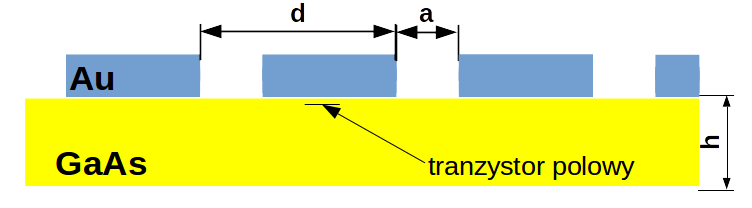
\includegraphics[width=\textwidth]{images/thz/schemat-podklad-falo.png}
	\caption{Schemat detektora promieniowania THz na tranzystorze polowym umieszczonym w falowodzie z $GaAs$ z naniesioną złotą siatką dyfrakcyjną}
	\label{fig:schem-podklad-falo}
\end{figure}

Rozkład pola na rysunku \ref{fig:consrcl525} nie zapewnia transportu promieniowania E-M w kierunku tranzystora polowego. W tym celu wykorzystany zostanie falowód tworzony przez podkład z $GaAs$. Siatka dyfrakcyjna tworząca antenę zostanie wykorzystana do dopasowania pędu fali padającej i pędu modu falowodowego. W tym celu należy rozwiązać równanie dyspersji modów falowodowych~\cite{petykiewicz1989podstawy}:
\begin{equation}
	\begin{gathered}
	\delta [ \kappa \textrm{cos}(\kappa h) + \gamma\textrm{sin}(\kappa h) ] - \kappa [ \kappa \textrm{sin}(\kappa h) - \gamma \textrm{cos}(\kappa h) = 0,\\
	\textrm{gdzie }\delta=\sqrt{\beta^2-\omega^2\mu_0\varepsilon_0},\textrm{ a }\kappa=\sqrt{\omega^2\mu_0 \varepsilon_0 \varepsilon_{\textrm{GaAs}}-\beta^2}.
	\end{gathered}
\end{equation}
Wszystkie wartości $\beta$ spełniające powyższą równość są dopuszczalnymi wartościami składowej wektora falowego w kierunku propagacji. W ten sposób efektywne współczynniki załamania modów TM w falowodzie planarnym można obliczyć jako $n_{\textrm{eff}}=\frac{\beta}{k_0}$. Rozwiązanie powyższego równania możliwe jest jedynie na drodze numerycznej~(lub graficznie). W przypadku rozważanych podkładów z $GaAs$, $h=400$~$\mu m$, możliwe wartości efektywnego współczynnika załamania przedstawia wykres \ref{fig:gaas-effn}. Różne współczynniki $n_{\textrm{eff}}$ odpowiadjące tej samej długości fali wynikają z wielomodowego charakteru falowodu tworzonego przez podkład $GaAs$. Na podstawie tych wyników przygotowano wykres zależności okresu siatki $d$ potrzebnej do wzbudzenia kolejnych modów falowodowych w zależności od długości fali dla której pracować ma antena. Założono prostopadłe oświetlenie struktury. Wyniki tych obliczeń przedstawia wykres \ref{fig:d-lusok}.

\begin{figure}
\begin{subfigure}{0.5\textwidth}
        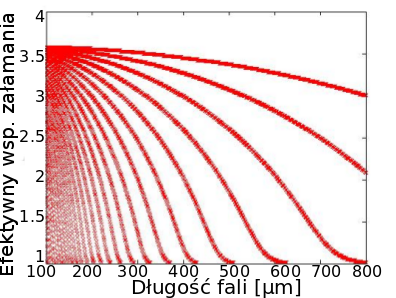
\includegraphics[width=\textwidth]{images/thz/gaas-neffeps.png}
	\caption{Zależność $n_{\textrm{eff}}$ od długości fali}
	\label{fig:gaas-effn}
\end{subfigure}
\begin{subfigure}{0.5\textwidth}
        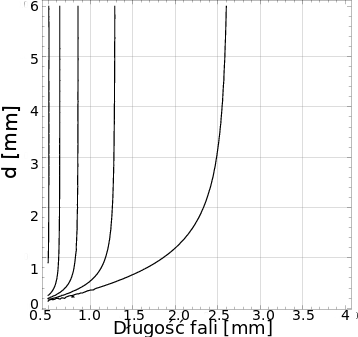
\includegraphics[width=\textwidth]{images/antenaThz/d_lambda.png}
	\caption{Wykres łączący okres siatki dyfrakcyjnej z długością fali dla której pracuje antena}
	\label{fig:d-lusok}
\end{subfigure}
\caption{Wyniki rozwiązania problemu falowodu planarnego o grubości $h=$400~$\mu$m z GaAs.}
\end{figure}



Na podstawie przeprowadzonych obliczeń zaproponowano siatkę dla źródła o częstotliwości $f=300$~GHz ($\lambda=1308$~$\mu$m) o grubości $H=1$~$\mu$m i okresie $d=729$~$\mu$m. W strukturach wytwarzanych eksperymentalnie pod podkładem $GaAs$ znajduje się warstwa $Au$ o grubości 1~$\mu$m, którą w symulacji metodą $FDTD$ traktujemy jako doskonały przewodnik. Na rysunku \ref{fig:consrc_1d_f300Ghz} przedstawiono rozkład gęstości energii wewnątrz zaproponowanej struktury. Wyniki symulacji komputerowych potwierdzają  możliwośc propagacji promieniowania E-M z zakresu subterahrecowego w kierunku detektora w zaprojektowanym układzie.

\begin{figure}[tb]
	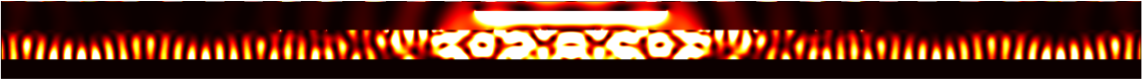
\includegraphics[width=\textwidth]{images/thz/consrc_siatka1d_300GHz_d729um.png}
	\caption{Uśredniony rozkład gęstości energii pola elektromagnetycznego wewnątrz falowodu z $GaAs$ na którym umieszczono antenę w postaci siatki dyfrakcyjnej o $d=$729~$\mu$m oświetloną pod kątem normalnym przy pomocy źródła o częstotliwości 300~GHz. Uzyskany przy pomocy symulacji metodą FDTD. }
	\label{fig:consrc_1d_f300Ghz}
\end{figure}

\begin{figure}
	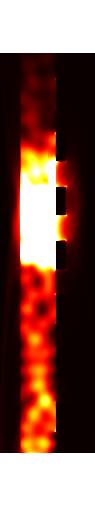
\includegraphics[width=0.2\textwidth, angle=90]{images/antenaThz/ro_consrc_radial_antena.png}
	%TODO: poprawcowac nad tym obrazkiem, ew. zrobic 3d
	\caption{!!!!!!!!!!!!!!!!!!!!!!!!!!1TEN RYSUNEK JEST DO ZMIANY, RAZEM Z OBRAZKIEM Z PARAGRAFU O BORFDTD!!!!!!!!!!!!!!!!!!!!!!!!!!!!!}	
	\label{fig:concent_modfalo}

\end{figure}




Bazując na pracach numerycznych dotyczących  jednowymiarowych siatek dyfrakcyjnych pozwalających na wzbudzenie modów falowodowych w podkładach z $GaAs$ przeanalizowane zostało działanie analogicznych falowodów opartych na cylindrycznych siatkach dyfrakcyjnych. Ze względu na wzbudzenie modów falowodowych o kierunku propagacji prostopadłym do pasków siatki dyfrakcyjnej uzyskujemy częściową koncentrację promieniowania w obszarze detektora. Odpowiedni eksperyment numeryczny został przeprowadzony przy użyciu metody FDTD we współrzędnych cylindrycznych, szerzej opisanej w podrozdziale \ref{subart:borfdtd}. Wyniki symulacji przedstawione na rysunku \ref{fig:concent_modfalo} odpowiada strukturze z $GaAs$ o rozmiarach 10x10mm pokrytej siatką dyfrakcyjną o okresie $d=538$~$\mu$m i otworach o szerokości $250$~$\mu$m (wspólczynnik wypelnienia ok. 0.53), która została oświetlona promieniowaniem o długosci fali $2.52$~mm.\footnote{Pozorny wzrost natężenia gęstości energii przy zbliżaniu się do środka struktury wynika ze zmniejszania elementu objetościowego wraz ze zbliżaniem do osi symetrii.} W ten sposób potwierdzono możliwośc wykorzystania tego typu struktur~\cite{Stolarek2011}.

